\documentclass[14pt]{extarticle}
\usepackage[left=2cm, top=3cm]{geometry}
\usepackage[utf8]{inputenc}
\usepackage{graphicx}
\usepackage{times}
\usepackage[czech]{babel}
\usepackage[breaklinks, unicode]{hyperref}
\usepackage{hyperref}
\usepackage{subfig}
\hypersetup{
    colorlinks=true
}


\begin{document}

	\begin{titlepage}
		\begin{center}
			
\includegraphics[scale=0.15]{fit_logo.png}
			\\
			\vspace{\stretch{0.152}}
			{\Large
				 \huge{{IMP 2021/2022 -- Projektová dokumentace\\[0.5em]}}}
				 \LARGE{Světelná tabule -- FITkit3\\}
			\vspace{\stretch{0.180}}
		{\LARGE
			\begin{tabular}{l c r}
            Vojtěch Fiala (xfiala61)
            \end{tabular}
			
		}
		\end{center}
	\end{titlepage}
	
	%\tableofcontents
	
	\newpage
	% úvod do řešené problematiky, popis způsobu a prostředků řešení a výsledky řešení.
    \section{Úvod}
    
    Cílem projektu bylo naprogramovat \uv{světelnou tabuli} za pomoci maticového 8x8 displeje (Celý displej je složen ze 2 kusů, tedy o celkové velikosti 16x8). Jako platforma bylo použito zařízení FITkit3. Projekt je napsán v jazyce C, pro vývoj bylo použito Kinetis Design Studio.
    
    Výsledkem projektu je program, který po nahrání do zařízení umožňuje uživateli si po zmáčknutí jednoho z 5 zvolených tlačítek nechat na displeji přehrát předem definovanou zprávu. Tato dokumentace se zabývá popisem implementace, funkcionality a základní teorií, která byla při tvorbě projektu využita.

    \subsection{Video}
     \label{uv}
    Prezentace řešení byla natočena skrz mobilní telefon a je umístěna na videoserveru Youtube, odkud je také přístupná skrz následující odkaz: \url{https://www.youtube.com/watch?v=SCR_aBKkG9Q}.

    \section{Příprava}
    
    Před začátkem samotné implementace projektu bylo nutno nastudovat základní informace o FITkitu pro realizaci zapínání a vypínání jednotlivých diod na maticovém displeji a způsob detekce zmáčknutí jednotlivých tlačítek.
    
    \subsection{Propojení maticového displeje s FITkitem}
    Konektor maticového displeje P3 je napojen na konektor P1 na FITkitu a pro obsluhu displeje se pak používají konkrétní piny portu P1 (které jsou inicializovány jako výstupní) -- \texttt{PTA6, PTA8, PTA10, PTA11 a PTE28} pro obsluhu vykreslování sloupců, což je realizováno za pomoci dekodéru 4 na 16 a poté piny \texttt{PTA7, PTA9, PTA24, PTA25, PTA26, PTA27, PTA28, PTA29}, které slouží pro vykreslování řádků. Jako hlavní zdroj informací o propojení sloužila prezentace k projektu \cite{project-info}.
    Na další stránce jsou k vidění ilustrace portů P1 a P3, které jsou převzaty (včetně popisu) z \cite{project-info}.
    
\begin{figure}
    \centering
    \subfloat[\centering Propojovací konektor P3 rozšiřujícího modulu s maticovými LED displeji]{{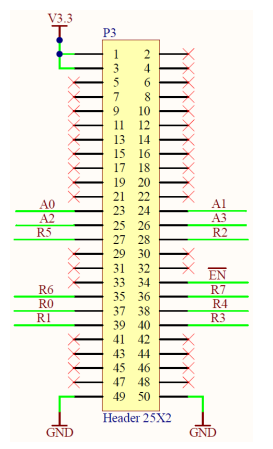
\includegraphics[width=5cm]{P3.png} }}%
    \qquad
    \subfloat[\centering Propojovací konektor P1 platformy FITkit]{{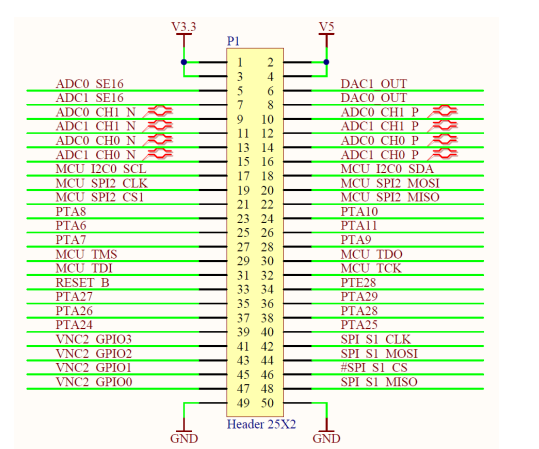
\includegraphics[width=9cm]{P1.png} }}%
    \caption{Schéma portů, skrz které jsou propojeny FITkit3 a maticový displej}%
\end{figure}
    
    \newpage
    \subsection{Detekce zmáčknutí tlačítka}
    Vstupní tlačítka jsou přístupná skrz porty \texttt{PTE10, PTE11, PTE12, PTE26 a PTE27}. Možností detekce zmáčknutí tlačítka  je více -- například sledovat, zda-li od nich nedošlo k vyvolání přerušení, nebo jednodušším a naivnějším přístupem kontrolovat stav pinů GPIOE PDIR registru (tlačítka se nachází v portu E) a porovnávat jej s bitem na pozici odpovídající jednotlivým tlačítkům.
    
    \subsection{Princip rozsvěcování světel}
    Aby bylo možno rozsvítit pouze konkrétní body, není možné pouze rozsvítit odpovídající sloupec a řádek, neboť by dříve nebo později došlo k tomu, že bude svítit i něco, co svítit nemá. Jako řešení tohoto problému jsem zvolil možnost založenou na principu použitém na 3. laboratorním cvičení z IMP. Jednotlivá světla tedy pouze jednou rozsvítím a hned poté zhasnu. Jelikož se takto však děje mnohokrát za vteřinu, lidské oko to vnímá, jako by světlo svítilo pořád. Samotné rozsvěcování světel probíhá za pomoci multiplexingu, kdy jsou určovány postupně sloupce a řádky, které mají svítit a jsou zapisovány do jednoho registru -- PTA Port Data Output Register (PDOR).
    
    \section{Řešení}
    Na začátek bych zde chtěl zmínit, že při tvorbě řešení jsem vycházel ze 2 již existujících programů -- primárně z ukázky funkcionality maticového displeje v programu\footnote{\url{https://wis.fit.vutbr.cz/FIT/st/cfs.php.cs?file=\%2Fcourse\%2FIMP-IT\%2Fprojects\%2FIMP_projekt+-+had_tabule_test.zip&cid=14662}} (včetně již naprogramovaného dekodéru 4 na 16), který vytvořil\break Ing. Václav Šimek a dále pak, v menší míře, z ukázkového demo programu\footnote{\url{https://wis.fit.vutbr.cz/FIT/st/cfs.php.cs?file=\%2Fcourse\%2FIMP-IT\%2Fexcs\%2FFITkit3-demo.zip&cid=14662}} k FITkitu3, který vytvořil Ing. Michal Bidlo, Ph.D. Tento fakt je uveden i ve zdrojových kódech projektu, kde jsou převzaté funkce přímo označeny.
    \\\\
    Nyní již k samotnému popisu řešení ---
    \\
    Projekt se skládá ze 3 souborů, konkrétně se jedná o soubory následující:
    \begin{itemize}
    \setlength\itemsep{1pt}
    \item \texttt{main.c} -- Hlavní řídící soubor.
    \item \texttt{letters.h} -- Hlavičkový soubor obsahující definice funkcí, které tvoří pole s písmeny.
    \item \texttt{letters.c} -- Implementace funkcí pro práci s písmeny.
    \end{itemize}
    
    Princip funkcionality řešení je takový, že existuje jedno velké 2D pole znaků typu \texttt{char} \uv{vysoké} 8 znaků a \uv{široké} až 64 znaků. Toto pole je následně naplněno jednotlivými písmeny, které se mají na displeji zobrazit. Jednotlivá písmena jsou definována jako pole znaků, opět typu \texttt{char}, o velikosti 8x8. Znak "1" v tomto poli definujícím vzor znaku znamená, že světlo na displeji má svítit, "0" pak znamená opak. Písmena jsou z estetického hlediska vysoká jen 7 z možných 8 znaků, protože s lichou výškou se dají namodelovet \uv{hezčí} písmena než s výškou sudou. Definice vzorů písmen jsou umístěny v souboru \texttt{letters.c} pro zpřehlednění čitelnosti kódu.
    
    Ve zdrojovém kódu je implementováno 5 různých textů, které se mají po zmáčknutí jednotlivých tlačítek na kitu vykreslit. Tento text (i se svou délkou) je předán funkci společně s prázdným polem a skrz jednotlivé písmena v textu je pole naplněno vzory písmen v takovém tvaru, v jakém mají být vykresleny na displeji.
    
    Po provedení předchozích kroků je tedy vytvořeno pole o šířce\linebreak \textit{délka\textunderscore textu * 8} složené ze znaků "1" a "0", které určují, jaká světla se mají na displeji rozsvítit. Následně probíhá iterace skrz toto pole, která je minimálně 2x větší, než je délka samotného textu, a to z důvodu, aby text tzv. \uv{odjel} za okraj a zničehonic z displeje nezmizel. V této smyčce je každá pozice pole vykreslena 12x, aby nedocházelo k nehezkému \uv{blikání}. Text se po displeji pohybuje tím způsobem, že je při jeho vykreslení použita i aktuální hodnota z vykreslovací smyčky, která značí posunutí, o které má být pole zobrazeno. 
    
    Jednotlivé tyto texty jsou, jak už bylo zmíněno, vykreslovány po zmáčknutí tlačítek na kitu. Pro detekci zmáčknutí jsem zvolil přístup, kdy program v hlavní smyčce kontroluje, zda bylo některé tlačítko zmáčknuto. Tyto funkce na detekci vycházejí z již zmíněného FITkit3 dema. Tento přístup detekce jsem zvolil z toho důvodu, že jsem byl neúspěšný v programování přerušení. Po detekci, že bylo tlačítko zmáčknuto, je tedy definován konkrétní text, co se má vykreslit a spuštěna vykreslovací smyčka. Po jejím skončení začně program opět kontrolovat, jestli došlo k dalšímu zmáčknutí tlačítka.
    
    \section{Výsledky}
    Výsledkem projektu je program, který po nahrání na kit umožňuje uživateli si po stisknutí jednoho z pěti předem určených tlačítek nechat na připojeném displeji přehrát určitou zprávu. Metoda řešení je funkční, mohla by však být efektivnější. Pro zvýšení elegance řešení by bylo možné například zajistit detekci stisknutí tlačítek skrz vyvolání přerušení či provádět překreslování displeje na základě časovače. K implementaci těchto zlepšení však z důvodu časové vytíženosti nedošlo. Výstupy projektu je možné vidět na demonstračním videu, které je umístěno v úvodní kapitole této dokumentace \ref{uv}.
    
    \newpage
    \section*{Dodatek}
    Dle zadání zde uvádím autoevaluaci složek E, F, Q, P, D.
    Subjektivně vnímám, že jsem body splnil následovně -- 
    \begin{itemize}
    \setlength\itemsep{0,5pt}
    \item \texttt{E} -- 0,5 -- Řešení by mohlo být efektivnější, žádná rozšíření nejsou, práce na projektu probíhala průběžně
    \item \texttt{F} -- 4 -- Projekt funguje, ale implementace mohla být efektivnější a využívat více modulů kitu
    \item \texttt{Q} -- 3 -- Kód považuji za čitelný a ovládání a výstupy za přímočaré
    \item \texttt{P} -- 1 
    \item \texttt{D} -- 4
    \end{itemize}
    
    \newpage
    \bibliographystyle{czechiso}
    \renewcommand{\refname}{Literatura}
    \bibliography{main}

\end{document}